\chapter{SPARK}
	In questo capitolo verrà analizzato \ac{SPARK}\index{SPARK}, il nostro attacco basato sul progetto SPECTRE capace di recuperare chiavi (o più in generale "segreti") evitando il controllo della password.
	
	\section{Scenario}
		Immaginiamo di partire dalla funzione attaccata da SPECTRE (\cref{list:vulnerabile}). Nello scenario più semplice si può pensare che \texttt{array1} (che d'ora in poi chiameremo \texttt{secret}) contenga delle chiavi predefinite assegnate ad ogni utente. Queste chiavi vengono utilizzate come indici  per accedere ad \texttt{array2}, che contiene le informazioni riservate di tutti gli utenti (ad esempio il saldo del conto corrente). Data la riservatezza di queste informazioni, l'accesso a questo array è protetto da una password. 
		
		L'utente \emph{x} che vorrà consultare i propri dati dovrà autenticarsi inserendo il proprio \texttt{userID} ed una password (salvata insieme alle password degli altri utenti nell'array \texttt{passwordDigest}). In caso di esito positivo del controllo, si utilizzerà il valore contenuto in \arr{secret}{userID} come indice di \texttt{array2} per andare a recuperare il dato sensibile riguardante x. In caso di esito negativo verrà ovviamente negato l'accesso ai dati.
		
		Tale funzione potrebbe essere implementata dal \cref{list:spark}:
		\codice{26}{30}{funzione attaccata da SPARK}{list:spark}
		
		Supponiamo adesso che l'attaccante abbia accesso ad \texttt{array2} (come supposto anche dall'attacco SPECTRE), ma che non abbia accesso all'array \texttt{secret} ed ovviamente neanche all'array delle password. L'obiettivo del nostro attacco è quello di ricavare, per un utente casuale \emph{x}, il relativo \arr{secret}{userID}, per poter successivamente avere accesso all'informazione riservata, il tutto senza conoscere la password.
		
		La precisione del risultato ottenuto dipende molto dal processore e dal tipo di dati utilizzato per rappresentare i diversi valori. Nella nostra implementazione abbiamo utilizzato il tipo primitivo \texttt{int} (dimensione 32 bit); questo, in una cache con dimensione delle line pari a $512$ bit (un valore considerato standard nei processori più moderni) non ci permette di recuperare esattamente \arr{secret}{x} (\cref{fig:lineSize}), tuttavia ci consente di localizzarlo in un intervallo di ampiezza $\delta$ con: $$\delta = \frac{\text{dimensione di una line}}{\text{dimensione del tipo di dato}} = \frac{512}{32} = 16.$$
		
		\begin{figure}
			\begin{center}
				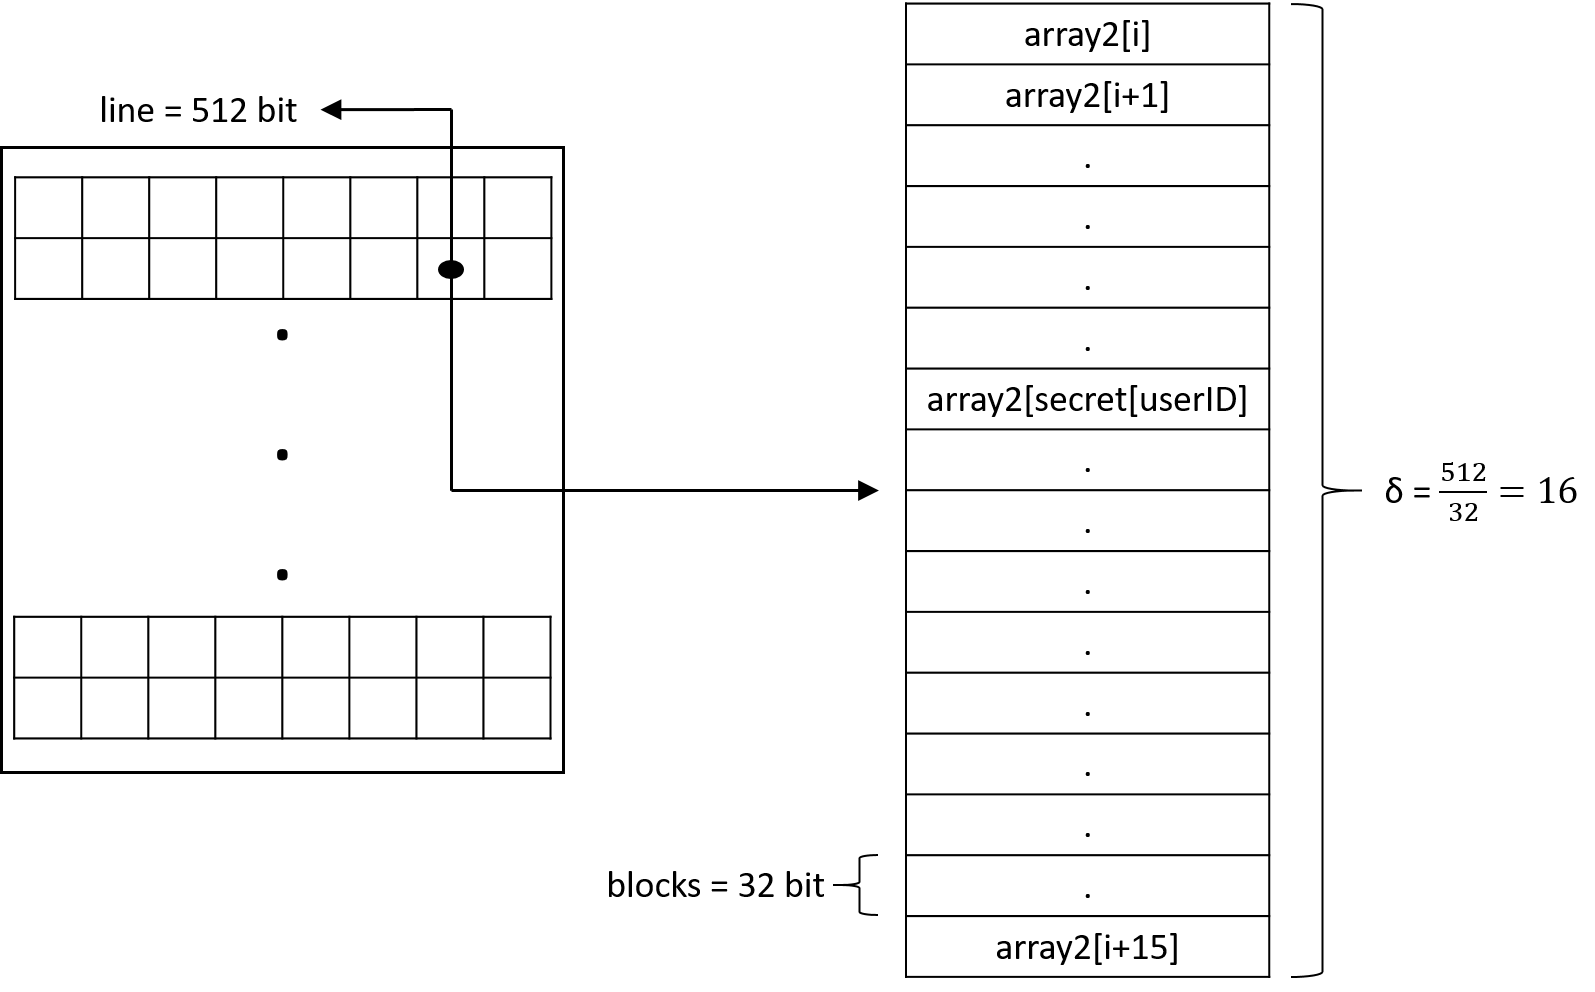
\includegraphics[width=.8\textwidth]{lineSize}
				\caption{contenuto di una cache line nel nostro setup}
				\label{fig:lineSize}
			\end{center}
		\end{figure}
		
		\section{L'attacco}
			Prima di analizzare l'effettiva implementazione, vediamo l'idea generale dell'attacco, che può essere schematizzato in quattro punti:
			
			\begin{enumerate}
				\item Il \ac{BP} viene addestrato richiamando la funzione vittima per tre volte con uno \texttt{userID} e la relativa password corretta. Per addestrare il BP, all'attaccante basterà semplicemente autenticarsi con i propri dati.
				\item Viene eseguito il \emph{flush} dalla cache di tutti i dati relativi ad \texttt{array2} e \texttt{passwordDigest}. Ricordiamo che l'istruzione \texttt{clflush} non richiede alcun privilegio per essere eseguita.
				\item Viene richiamata la funzione vittima con lo \texttt{userID} di cui vogliamo scoprire il segreto (che nel codice chiameremo \texttt{userUnderAttack}) ed una password casuale.
				\item Viene calcolato il tempo necessario ad accedere ad alcune posizioni di \texttt{array2}. Considerato che, data l'esecuzione speculativa dovuta alla chiamata precedente, l'unico dato relativo ad \texttt{array2} presente in cache in questo momento è \emph{y} = \arrdoppio{array2}{secret}{userUnderAttack}, otterremo un tempo basso solamente per una posizione presente nella stessa line che contiene \emph{y}. Per tutte le altre invece sarà alto in quanto il dato dovrà essere recuperato dalla memoria principale.
			\end{enumerate}
		
			Questo attacco sfrutta l'esecuzione speculativa del processore sul controllo della password. Infatti, avendo eseguito il \emph{flush} di \texttt{passwordDigest} al punto due, \emph{z} = \arr{passwordDigest}{userUnderAttack} non sarà presente in cache al momento del controllo al punto tre. Nell'attesa del suo recupero dalla memoria principale, il \ac{BP} eseguirà il ramo then della computazione a causa dell'addestramento ottenuto al punto uno. Il valore di \emph{y} verrà quindi prelevato dalla memoria e messo nella cache. Quando sarà disponibile \emph{z}, il controllo fallirà e non verrà permesso l'accesso ai dati, ma \emph{y} resterà in cache. A questo punto, accedendo a varie posizioni di \texttt{array2}, l'unica ad avere un tempo di accesso veloce sarà quella che ci dirà quale line contiene il segreto. La scelta delle posizioni da accedere e il calcolo del range viene spiegato più dettagliatamente nella prossima sezione.
			
			\subsection{Implementazione}
				Passiamo adesso all'analisi vera e propria del nostro programma che implementa l'attacco.
				
				\subsubsection{Inizializzazione}
				\codspark{1}{18}{inizializzazione}
				
				Nella primissima parte vengono semplicemente caricate le librerie necessarie alla compilazione, viene definito il numero di utenti (tremila), vengono creati i tre array principali (\texttt{secret}, \texttt{array2} e \texttt{passwordDigest}) e viene definita la funzione vittima, esattamente la stessa proposta nello scenario.
				
 				La libreria \texttt{x86intrin} fornisce le istruzioni \texttt{rdtscp} e \texttt{\_\_mm\_clflush} necessarie al calcolo dei tempi di hit e al flush della cache. In particolare l'istruzione \texttt{\_\_mm\_clflush} prende come argomento un indirizzo di memoria ed invalida, su tutti i livelli della cache, tutte le line che contengono quell'indirizzo.
				
				I tre array "utili" sono separati da altri array \texttt{unused} per essere sicuri che vengano distanziati in memoria. Questo fa sì che non si sovrappongano all'interno di una stessa line.
				
				\subsubsection{Main - definizione parametri}
				\codspark{19}{39}{main - definizione parametri}
				
				In questa parte vengono definiti i parametri che verranno utilizzati nel resto del programma:
				
				\begin{itemize}
					\item \texttt{CACHELINE}: la dimensione in bit di una singola cache line. Come già detto, questa dimensione è ormai standardizzata a $512$ bit su tutti i processori moderni.
					
					\item \texttt{blocks}: la dimensione in bit di un singolo elemento dell'array. In questo caso 32 bit.
					
					\item \texttt{delta}: il numero di elementi dell'array contenuti in una cache line.
					
					\item \texttt{class}: il numero di posizioni da controllare per coprire tutto \texttt{array2} con uno step pari a $\delta$. Questo valore fornisce anche il numero di line occupate in cache da \texttt{array2}.
					
					\item \texttt{numberOfRuns}: il numero di volte che viene eseguito l'attacco per ogni esperimento.
					
					\item \texttt{numberOfTests}: il numero di esperimenti che vengono eseguiti.
					
					\item \texttt{cacheHitThreshold}: la soglia entro la quale il tempo calcolato viene considerato una cache hit. Sperimentalmente questo valore si aggira tra i trenta e i quaranta cicli di clock, ma dipende dalla latenza della particolare cache attaccata.
					
					\item \texttt{precisionLoss}: con questo valore si regola la precisione che si vuole ottenere. Se lasciato a zero verrà restituito un intervallo di ampiezza $\delta$ che dovrebbe contenere il segreto. A volte però può succedere che l'intervallo calcolato non contenga il segreto a causa di interferenze con altri processi che utilizzano il processore, o a causa di un diverso allineamento delle cache. Aumentando questo valore si aumenta l'ampiezza dell'intervallo proporzionalmente a $\delta$, perdendo un po' in localizzazione, ma guadagnando in correttezza dell'intervallo (questo, insieme a \texttt{numberOfRuns}, \texttt{numberOfTests} e \texttt{cacheHitThreshold} sono i quattro parametri richiesti all'avvio del programma).		
								
					\item \texttt{results}: l'array nel quale verrà salvato il numero di hit rilevate per ogni line di cache.
					
					\item \texttt{ok}, \texttt{error} e \texttt{no-hit}: tre contatori utilizzati rispettivamente per sapere quante volte il programma restituisce l'intervallo che contiene il segreto, quante volte lo restituisce sbagliato e quante volte non rileva nessun cache hit.
					
					\item \texttt{timeReg}, \texttt{time1} e \texttt{time2}: le tre variabili per calcolare i tempi di accesso alle posizioni di \texttt{array2}.
				\end{itemize}			
				Dopo aver definito tutti i parametri, si procede con l'inizializzazione del generatore \texttt{srand()} di numeri casuali.
				
				\subsubsection{Main - inizializzazione dell'esperimento}
				\codspark{40}{51}{main - inizializzazione dell'esperimento}
				
				All'inizio di ogni test viene scelto casualmente lo \texttt{userUnderAttack} e vengono inizializzati casualmente i tre array principali \texttt{passwordDigest}, \texttt{array2} e \texttt{secret}. Successivamente si sceglie una password sicuramente sbagliata ed infine si prepara l'array \texttt{results} al conteggio delle hit settandolo a zero.
				
				\subsubsection{Main - l'attacco}
				\codspark{52}{71}{main - l'attacco}
				
				Come descritto nello scenario, l'attacco si divide in quattro parti. Nella prima parte viene addestrato il \ac{BP} ad eseguire speculativamente il ramo then della funzione vittima, richiamandola per tre volte con \texttt{userID} e password corretta.
				
				Successivamente si esegue il flush dalla cache di tutte le posizioni degli array \texttt{array2} e \texttt{passwordDigest}.
				
				Prima di richiamare la funzione vittima facciamo eseguire l'istruzione \texttt{\_mm\_lfence}. Tale istruzione è una barriera sulla memoria che non permette l'esecuzione delle istruzioni successive prima che siano terminate tutte le scritture in memoria delle istruzioni precedenti. Questo evita ad esempio che l'istruzione a riga $90$ venga eseguita prima del flush di \texttt{array2} a causa di un riordinamento del codice. Se accadesse questo, il risultato del calcolo del tempo di accesso sarebbe ovviamente falsato.
				
				Terminato il flush della cache, viene richiamata la funzione vittima e vengono calcolati i tempi di accesso alle varie posizioni di \texttt{array2}. Come si può notare, non si effettua l'accesso a tutte le posizioni di \texttt{array2} ma si procede con un passo $\delta$ visto che una qualunque delle $\delta$ posizioni all'interno della line che contiene il segreto restituirà comunque una hit.
				
				Con un'altra \texttt{\_mm\_lfence} ci assicuriamo che il tempo venga effettivamente salvato in \texttt{time2} ed effettuiamo il controllo. Se il risultato del calcolo del tempo di accesso è minore della soglia che abbiamo impostato, aumentiamo di uno nell'array \texttt{results} il valore  contenuto all'indice che stiamo analizzando.
				
				\subsubsection{Main - i risultati}
				\codspark{72}{105}{main - i risultati}
				
				\begin{figure}[b]
					\begin{center}
						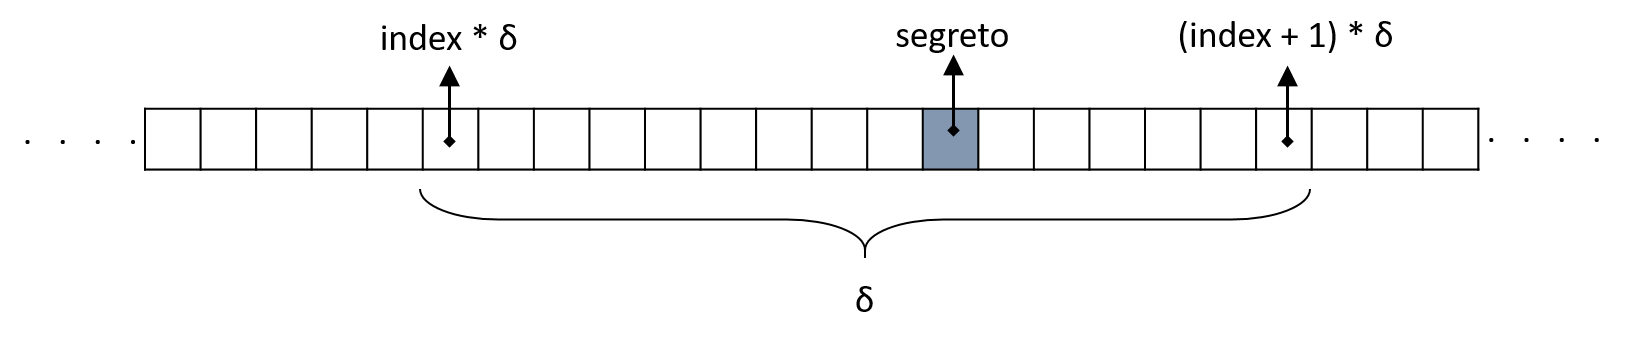
\includegraphics[width=\textwidth]{range}
						\caption{calcolo del range}
						\label{fig:range}
					\end{center}
				\end{figure}
				
				Nell'ultima parte del programma viene cercato l'indice \texttt{index} con il valore più alto nell'array \texttt{results}. Questo indice rappresenta la porzione di \texttt{array2} che dovrebbe contenere il segreto. Da questo indice viene calcolato il range da restituire (\cref{fig:range}) limitato in basso da $0$ ed in alto da \texttt{SIZE} che non è altro che: $$((index - precisionLoss) * \delta\ ,\ (index + 1 + precisionLoss) * \delta).$$ Il risultato così ottenuto viene infine comparato con \arr{secret}{userUnderAttack} e viene stabilito il risultato dell'attacco:
				
				\begin{itemize}
					\item \texttt{OK} - se il segreto ricade nel range calcolato.
					\item \texttt{ERROR} - se il segreto non ricade nel range calcolato.
					\item \texttt{NO-HIT} - se non si è rilevata alcuna hit.
				\end{itemize}
				
				Come ultima cosa viene visualizzato sullo schermo un resoconto dei risultati ottenuti. Nella \cref{fig:schermata} si può vedere la schermata del programma.
				
				\begin{figure}
					\begin{center}
						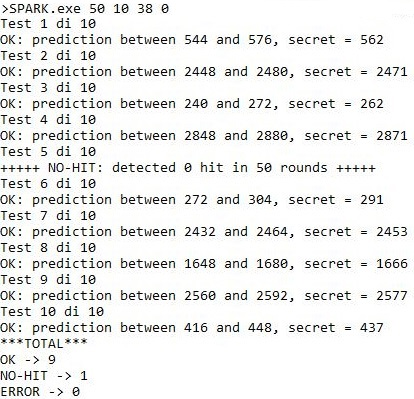
\includegraphics[width=.6\textwidth]{risultati}
						\caption[schermata di SPARK]{schermata del programma lanciato con i parametri $50,100,38,0$}
						\label{fig:schermata}
					\end{center}
				\end{figure}
			
			\subsection{Prove sperimentali}
				Abbiamo testato il programma su un notebook SAMSUNG-R$580$ che monta un processore INTEL CORE i$3$-$330$M a $2.13$\gigahertz e su un computer desktop equipaggiato con un processore i$7$-$4700$MQ a $2.40$\gigahertz. Di seguito i risultati ottenuti con ognuno dei due.
				
				\subsubsection*{INTEL CORE i$3$-$330$M} 
				
					Questo processore dispone di tre livelli di cache così suddivisi:
					
					\begin{itemize}
						\item [L$1$ -] $2$ x $64$ \kilobyte \ divise in 
						\begin{itemize}
							\item  $2$ x $32$ \kilobyte \ $4$-way associative cache per i dati
							\item  $2$ x $32$ \kilobyte \ $8$-way associative cache per le istruzioni
						\end{itemize}
						\item[L$2$ -] $2$ x $256$ \kilobyte \ $8$-way associative cache
						\item[L$3$ -] $3$ \megabyte \ $12$-way associative cache condivisa dai due core
					\end{itemize}
				
					\begin{figure}
						\begin{center}
							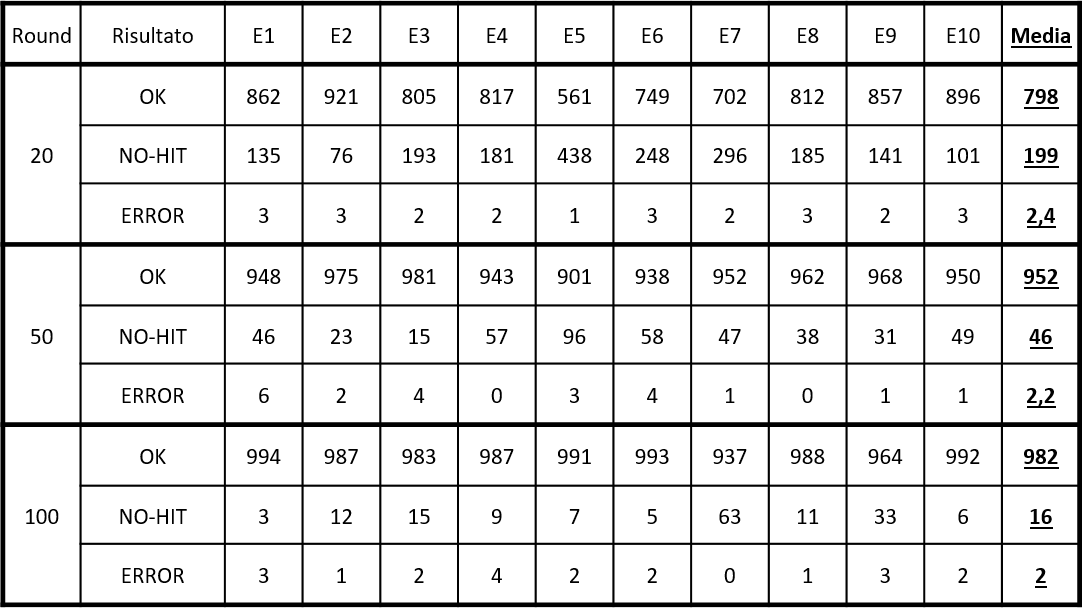
\includegraphics[width=\textwidth]{risultatiTab}
							\caption{risultati ottenuti sul processore i$3$-$330$M}
							\label{fig:risultati}
						\end{center}
					\end{figure}
				
					Abbiamo effettuato dieci sessioni di esperimenti (i cui risultati sono visibili in \cref{fig:risultati}), ognuna composta da tremila test suddivisi in:
					
					\begin{itemize}
						\item mille in cui vengono eseguiti venti run ogni test
						\item mille in cui vengono eseguiti cinquanta run ogni test
						\item mille in cui vengono eseguiti cento run ogni test.
					\end{itemize}
					
					Come è normale aspettarsi, maggiore è il numero di round effettuato per ogni test, maggiore è la precisione che si ottiene. Nei nostri esperimenti si passa infatti da una media di successi ottenuti del $79.8\%$ con venti round a $98.2\%$ con cento round. Ovviamente, aumentando il numero di round, aumenta il tempo di esecuzione che nei due casi precedenti passa, per ogni test, da meno di un secondo a circa cinque secondi.
					
				\subsubsection*{INTEL CORE i$7$-$4700$MQ} 
				
					Anche questo processore dispone di tre livelli di cache così suddivisi: 
					
					\begin{itemize}
						\item [L$1$ -] $4$ x $64$ \kilobyte \ divise in 
						\begin{itemize}
							\item  $4$ x $32$ \kilobyte \ $8$-way associative cache per i dati
							\item  $4$ x $32$ \kilobyte \ $8$-way associative cache per le istruzioni
						\end{itemize}
						\item[L$2$ -] $4$ x $256$ \kilobyte \ $8$-way associative cache
						\item[L$3$ -] $6$ \megabyte \ $12$-way associative cache condivisa dai quattro core
					\end{itemize}
					
					\begin{figure}
						\begin{center}
							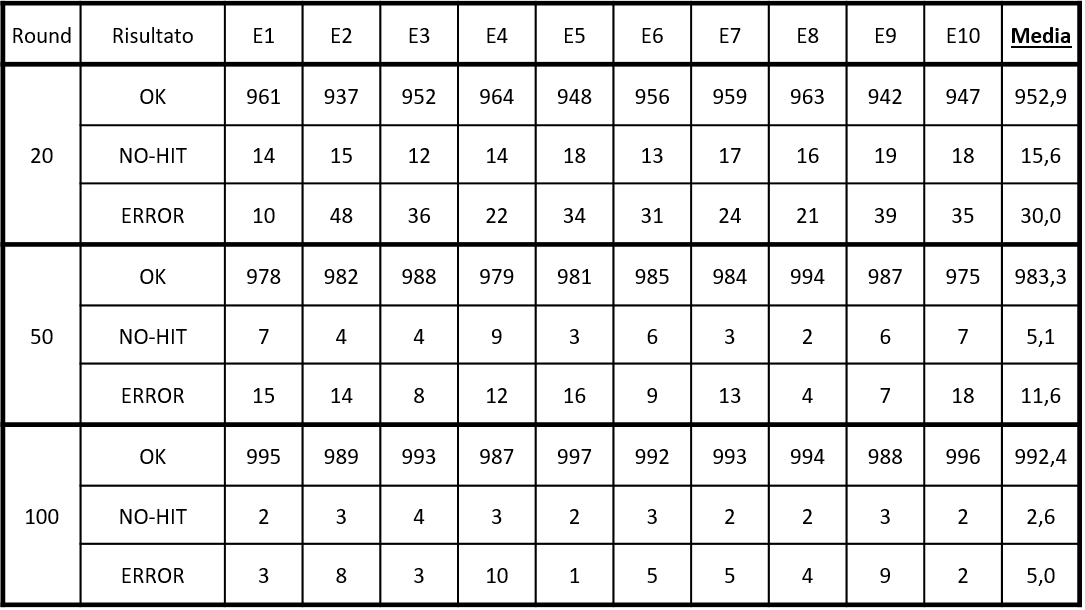
\includegraphics[width=\textwidth]{risultatiTab2}
							\caption{risultati ottenuti sul processore i$7$-$4700$MQ}
							\label{fig:risultati2}
						\end{center}
					\end{figure}
					
					Anche in questo caso abbiamo effettuato dieci sessioni di esperimenti (i cui risultati sono visibili in \cref{fig:risultati2}), esattamente identiche alle precedenti.
					
					Le indicazioni ottenute sono in linea con i test eseguiti sull'altro processore con una precisione che aumenta all'aumentare del numero di round. In questo caso si parte infatti da una media di successi ottenuti del $95.3\%$ con venti round fino ad arrivare al $99.2\%$ con cento round. Utilizzando un processore con prestazioni migliori, i tempi di esecuzione si sono sensibilmente abbassati: si passa da circa $0.4$ secondi a test se effettuati con venti round a $2$ secondi a test se effettuati con cento round (circa il doppio più veloce del precedente).
					
					Anche il maggior numero di errori è molto probabilmente dovuto alle migliori prestazioni del processore. Trattandosi di un computer general purpose, equipaggiato con Windows $10$ come sistema operativo, nel tempo di esecuzione del programma altri processi possono interagire con la cache creando così delle false hit. 
					
					Sarebbe interessante eseguire questi esperimenti su macchine dedicate esclusivamente all'esecuzione di questo programma per capire quanto l'influenza di processi esterni possa interferire con l'esecuzione di SPARK. 
					